\documentclass[a4paper, openright, twoside]{report}
\usepackage[utf8]{inputenc}
\usepackage[american]{babel}
\usepackage{hyphenat}
\usepackage[activate={true,nocompatibility}, final, tracking=true, kerning=true, factor=1100, stretch=10, shrink=10]{microtype}
% Prevent hyphenization
\tolerance=1
\emergencystretch=\maxdimen
\hyphenpenalty=10000
\hbadness=10000

\usepackage[hmarginratio=1:1,textwidth=360pt,textheight=595.8pt]{geometry}
% Packages
\usepackage{import}

% Math
\newcommand\hmmax{0}
\newcommand\bmmax{0}
\usepackage{bm}
\usepackage{amsmath, amsfonts, amssymb, mathrsfs,extarrows}
\usepackage{commath}
\usepackage[retainorgcmds]{IEEEtrantools}
\usepackage{siunitx}
\usepackage{multirow}
\usepackage[widespace]{fourier}

% Tables
\usepackage{array}
\usepackage{caption}
\usepackage[figuresright]{rotating}
\usepackage{multirow}
\usepackage{makecell}
\usepackage{footnote}
\makesavenoteenv{tabular}

% Algorithm
\usepackage[chapter]{algorithm}
\usepackage{algpseudocode}

%% Citations
\usepackage[numbers]{natbib}
\bibliographystyle{humannat}
\citestyle{egu}
\usepackage[hyphens]{url}
% Bibliography showing in TOC
% \usepackage[nottoc,numbib]{tocbibind}
\usepackage[nottoc]{tocbibind}
\usepackage{scrlayer}
\DeclareNewLayer[
    foreground,
    %textarea,% use only the textarea
    contents={%
      \parbox[b][\layerheight][c]{\layerwidth}
        {\centering Page intentionally left blank.}%
    }
  ]{blankpage.fg}
\DeclarePageStyleByLayers{blank}{blankpage.fg}

% Control structures
\usepackage{ifthen}

% Listing
\usepackage{listings}
\usepackage{xcolor}
\usepackage{float}

% Review notes:
\usepackage{xargs}
\usepackage[textwidth=30mm,textsize=footnotesize]{todonotes} % to create comments (useful to your advisor!)
\newcommandx{\bpf}[2][1=]{\todo[linecolor=blue,backgroundcolor=blue!25,bordercolor=blue,#1]{#2}} % Bernardo notes

% Equation color background
\usepackage{mdframed}

\newmdenv[
    hidealllines=true,
    backgroundcolor=black!20,
    skipbelow=\baselineskip,
    skipabove=\baselineskip
]{highlight}

\newcounter{problem}[chapter]\setcounter{problem}{1}
\renewcommand{\theproblem}{\arabic{chapter}.\arabic{problem}}
\newenvironment{problem}[2][]{%
    \refstepcounter{problem}

    \mdfsetup{hidealllines=true,
    backgroundcolor=black!20,
    skipbelow=\baselineskip,
    skipabove=\baselineskip,
    frametitle={Problem~\theproblem~|~#1}}

\begin{mdframed}[]\relax}{%
\end{mdframed}}

% Enumeration
\usepackage{enumerate}


% Images
\usepackage[labelformat=simple]{subcaption}
\renewcommand\thesubfigure{(\alph{subfigure})}
\renewcommand\thesubtable{(\alph{subtable})}
\usepackage{graphicx}
\graphicspath{ {figures/} }
\usepackage{array}
\usepackage[section]{placeins}
\usepackage{color}
% \usepackage{subcaption}
% \usepackage{subfig}



% Images SVG
\usepackage{import}
\usepackage{xifthen}
\usepackage{pdfpages}
\usepackage{transparent}

\newcommand{\incfig}[1]{
    \def\svgwidth{0.3\columnwidth}
    \import{images/studies/minkowski/fundamental_forms_2D/}{#1.pdf_tex}}


% Floating environment for listings
\floatstyle{plain}
\newfloat{lstfloat}{htbp}{lop}[chapter]
\floatname{lstfloat}{Listing}
\def\lstfloatautorefname{Listing} % needed for hyperref/auroref

% Listing style
\definecolor{codegreen}{rgb}{0,0.6,0}
\definecolor{codegray}{rgb}{0.5,0.5,0.5}
\definecolor{codepurple}{rgb}{0.58,0,0.82}
\definecolor{backcolour}{rgb}{0.95,0.95,0.92}

\lstdefinestyle{mystyle}{
    backgroundcolor=\color{backcolour},
    commentstyle=\color{codegreen},
    keywordstyle=\color{blue},
    numberstyle=\tiny\color{codegray},
    stringstyle=\color{codepurple},
    basicstyle=\fontsize{7}{10}\selectfont,
    breakatwhitespace=false,
    breaklines=false,
    captionpos=b,
    keepspaces=true,
    numbers=left,
    numbersep=5pt,
    showspaces=false,
    showstringspaces=false,
    showtabs=false,
    tabsize=2
}

\lstset{style=mystyle}

\makeatletter
\newcommand*{\shifttext}[2]{%
  \settowidth{\@tempdima}{#2}%
  \makebox[\@tempdima]{\hspace*{#1}#2}%
}
\makeatother

\usepackage{pythonhighlight}

% Appendices
\usepackage[toc,page]{appendix}

% Headers and footers
\usepackage{fancyhdr}
% \renewcommand{\chaptermark}[1]{\markboth{\thechapter.\ #1}{}}
% \renewcommand{\sectionmark}[1]{\markright{\thesection.\ #1}}

% \fancypagestyle{plain}{
% \fancyhf{}
% \fancyhead{}% remove default header entries
% \fancyhead[RE]{a\textsc{\leftmark}}
% \fancyhead[LE]{\thepage}
% \fancyhead[LO]{\textsc{\rightmark}}
% \fancyhead[RO]{\thepage}
% \renewcommand{\headrulewidth}{0.1pt} }
% \pagestyle{plain}

\fancypagestyle{firststyle}
{
   \fancyhf{}
    \fancyhead{}% remove default header entries
   \fancyfoot[C]{Porto, September 2021}
   \renewcommand{\headrulewidth}{0pt}
\renewcommand{\footrulewidth}{0.1pt}
    \fancyfootoffset{-0.25\textwidth}
}

\pagestyle{fancy}
\fancyhf{}
\renewcommand{\chaptermark}[1]{\markboth{\thechapter.\ #1}{}}
\renewcommand{\sectionmark}[1]{\markright{\thesection.\ #1}}
\fancyhead{}% remove default header entries
\fancyhead[RE]{\nouppercase\leftmark}
\fancyhead[LE]{\thepage}
\fancyhead[LO]{\nouppercase\rightmark}
\fancyhead[RO]{\thepage}
\renewcommand{\headrulewidth}{0.1pt}

\newenvironment{dedication}
  {%\clearpage           % we want a new page          %% I commented this
   \thispagestyle{empty}% no header and footer
   \vspace*{\stretch{1}}% some space at the top
   \itshape             % the text is in italics
   \raggedleft          % flush to the right margin
  }
  {\par % end the paragraph
   \vspace{\stretch{3}} % space at bottom is three times that at the top
   \clearpage           % finish off the page
  }


% landscape
% \usepackage{lscape}
\usepackage{pdflscape}

%Custom FramedBox Environment
%%Loading 'float' package
\usepackage{float}
%%Customize 'boxed' float style (caption above the body)
\makeatletter
\newcommand\fs@boxedtop
 {\fs@boxed
  \def\@fs@mid{\vspace\abovecaptionskip\relax}%
  \let\@fs@iftopcapt\iftrue
 }
\makeatother
%%Defining float commands
\floatstyle{boxedtop}
\floatname{framedbox}{Box}
\newfloat{framedbox}{hbt}{lob}[chapter]

% Symbols
%% Differential Upright "d"
\newcommand{\ud}{\,\mathrm{d}}
%% Assemble operator
\DeclareMathOperator*{\assemble}{\text{\Large $ \mathsf{A} $}}
%% Matrices and vectors
\newcommand{\vect}[1]{\bm{#1}}
\newcommand{\mat}[1]{\bm{#1}}
\newcommand{\boldsf}[1]{\boldsymbol{\mathsf{#1}}}

\DeclareMathAlphabet{\pazocal}{OMS}{zplm}{m}{n}

\title{Numerical Methods}
\author{José Luís Passos Vila-Chã}
\date{May 2021}


\pagenumbering{roman}

%Hypertext marks
\usepackage[pdftitle={NLMFEA_assignment},
			pdfauthor={JoseVila-Cha},
			pdfdisplaydoctitle=true,
			colorlinks=true,
			% Eletronic Version
             linkcolor=orange,
             citecolor=teal,
            % Print Version
            % linkcolor=black,
            % citecolor=black,
            bookmarks=true,
            bookmarksopen=false,
            bookmarksnumbered=true]{hyperref}

\usepackage[intoc]{nomencl}
\usepackage{xstring}
\usepackage{xpatch}
\patchcmd{\thenomenclature}
  {\leftmargin\labelwidth}
  {\leftmargin\labelwidth\itemindent 1em }
  {}{}

% Nomenclature

\makenomenclature
\renewcommand{\nomname}{Notation}
%% This code creates the groups
% -----------------------------------------
\usepackage{etoolbox}
\newcommand{\nomenclheader}[1]{%
  \item[\hspace*{-\itemindent}\bfseries\LARGE#1\vphantom{$\Bigg \vert $}]}
\renewcommand\nomgroup[1]{%
  \IfStrEqCase{#1}{%
   {A}{\nomenclheader{General abbreviations}}%      A - Acronyms
   {N}{\nomenclheader{General notation}}% R - Roman
   {O}{\nomenclheader{Operators and symbols}}% G - Greek
   {D}{\nomenclheader{Sets, domains and boundaries}}% G - Greek
   {S}{\nomenclheader{Subscripts and superscripts}}%  S - Superscripts
   {C}{\nomenclheader{Accents}}%    U - Subscripts
   {V}{\nomenclheader{Variables}}% X - Other Symbols
  }%
  \vspace{20pt}
}
\setlength{\nomitemsep}{-1pt}
% -----------------------------------------



\begin{document}
\begin{titlepage}
\thispagestyle{firststyle}
\begin{center}
   \begin{minipage}[c][10cm][l]{0.9\textwidth}

        
\includegraphics[width=0.6\textwidth]{figures/university}

        \vspace{3.5cm}
        \huge
       \textbf{FFT-based Homogenization Methods}

       \vspace{1.5cm}
        \small
       \textit{Professor:}\\
       \normalsize
       Francisco Manuel Andrade Pires 	\\

       \vspace{0.5cm}


         \small
        \textit{Student:}\\
        \vspace{0.5cm}
       \normalsize
       \!José Luís Passos Vila-Chã
       \vspace{8cm}


        \centering
       \small
       Report presented under the scope of the\\ Doctoral Program in Mechanical Engineering

   \end{minipage}
   \end{center}
\end{titlepage}

\newpage\null\thispagestyle{blank}\newpage

\setcounter{tocdepth}{2}
\tableofcontents


\listoffigures


\listoftables

\newpage\null\thispagestyle{blank}\newpage

\pagenumbering{gobble}
\pagenumbering{arabic}
\pagestyle{fancy}
% \chapter{Introduction}

\section{Motivation}

The present work presents a partitioned thermomechanical solver.

The current work focuses on the developement of an implicit partitioned thermomechanical solver.

It presents a comprehensive dissertation on the thermodynamically consistent continuum mechanics.
It follows with the strictly mechanical problem, the strictly thermal problem and the full thermomechanical problem.
The corresponding intial value problems for the constitutive problem are introduced, as is the weak formulation of the relevant conservation and balance principles and their spatial and temporal discretization.

It follows a validation of the thermal solver.
The mechanical solver is not validated as it is part of the LINKS code used as the basis for the current developments.
Appropriate references are used in DIN 1992 and the NAFEMS benchmarks.
There is a good agreement between the numerical results and the references.

It follows a thorough investigation on the available approaches to solve coupled problems, with a special focus on thermomechanical problems.
A large sweep of the literature is performed, with the main classes of solution procdures being the monolithic approaches and the partitioned approaches.
The partioned approaches can be further divided into loosely coupled or explicit and strongly coupled or implicit.
Given the requirements put forth the most promising solution is determined to be a strongly coupled or implicit partitioned scheme.

Having performed this choice the following step is to understand the implicit methods available.
Recasting the problem as a system of nonlinear equations, where the residual is the difference bewteen the initial input and its output after applying the fixed-point.
This approach leads to the consideration of a large family of methods for the solution of nonlinear equations.
These are presented in detail for the solution of coupled multi-physics systems.
These are the fixed-point method, the underrelaxation method, the Aitken relaxation, the Broyden-like family of methods, the Newton-Krylov methods and the polynomial vector extrapolation methods, MPE and RRE, in cycling mode.

The validation of the thermomechanical solver and the implicit solution methodsm, as well as their comparison, is performed using to examples, whose results are present in the literature.
The expansion of an infinitely long thick-walled thermoelastic cylinder, and the necking of circular thermoelastoplastic bar.
The numerical results agree with the references provided confidence in the solution developed.
Regarding the comparison of the different implicit techniques, the best performing are the Broyden-like methods with \(\beta=-1\), Type I update and \(s=1\), corresponding to the good Broyden method, and \(s=2\).
These are both computationally efficient with few calls to the residual function and not very memory intensive.
The Aitken relaxation being the simplest and the least memory intensive also performs well.
The other methods considered, including the Newton-GMRES and the MPE in cycling mode, display a worse performance.
There is however a caveat regarding the Newton-Krylov methods regarding the possible use of global strategies such as line search given the accurate estimate for the Jacobian of the residual.
Moreover, it has been determined that most computationally demanding portion of the implicit partitioned schemes is the solution of the mechanical and thermal problems, with the manipulation concerning solely the coupling solver taking a very minute portion of the total computational time.



% The goal of computational micromechanics of materials is to establish a link between the mechanical response of two interacting scales in heterogeneous media, commonly referred to as the macro and micro-scale.
% It generally involves the numerical solution of the mechanical equilibrium of a periodic unit cell.
% It is a boundary value problem defined on a representative microscale sample that involves local constitutive laws, balance equations, and, most typically, periodic boundary conditions.
% The solution of this problem plays a pivotal role in bridging the two scales considered.
% The effective macroscopic response is then extracted from the solution of the local problem for a given macroscopic excitation.

Many processes use temperature.
There is a tigh connection between the thermal and the mechanical fields.

Having properly formulated the thermomechanical problem in a thermodynamically consistent way the problem can be solved using the Finite Element Method for the spatial discretizaiton and some other thing for the time discritization.

A thermal solver can be easily implemented to solve solely thermal problems.

To solve the fully thermal problem there are two common approaches, the monolithic approach where the balance equations considered after the discretization are the balance of mechanical and conservation of energy, and a partitioned approach, where the problems are solved speratly.
Whithin this scheme, one can still find loosley or explicit approach or a strongly coupled or implicit approach.
Both strategies can be found in the literature, having both their benifits and drawbacks.

% 
% For virtually all cases of practical relevance, the local problem must be solved approximately by discretizing the microstructure and the unknown microscopic fields.
% Such a unit-cell thereby provides a representative geometrical representation of the microstructure - which is often complex.
% An accurate representation of reality, therefore, necessitates a high-resolution numerical method, which remains efficient in three dimensions.
% The prevailing technique employed for this purpose is the Finite Element Method.
% However, the ever-increasing desire to use finely discretized unit cells, even in 3D, calls for more efficient methods.
% In particular, advances in experimental characterization of microstructures by high-resolution images triggers the need for efficient solvers that use these images directly as computational grids.
% A regular grid in combination with periodic boundary conditions naturally promotes solvers based on the Fast Fourier Transform (FFT) \citep{zeman_finite_2017, de_geus_finite_2017}.
% An attractive competitor to the Finite Element Method was developed by \cite{moulinec_fast_1994, moulinec_fft-based_1995}.
% It employs the Fast Fourier Transform (FFT) to obtain a significant gain in efficiency compared to Finite Elements, both in terms of speed and in terms of memory footprint.
% In the meantime extensions and different FFT-based approaches have been proposed.
% This work pretends to give an overview of the relevant literature on FFT-based homogenization procedures.
% 
% The improvements in efficiency obtained using the FFT-based procedures are of special relevance in the context of the data-driven design of materials, where the number of mechanical simulations needed to populate the database can be very large.
% Structural and material design is a highly iterative process where an optimal design for a chosen set of quantities of interest and a given set of restrictions is sought.
% For the particular case of material systems design, the high dimensionality of the engineering design space is striking when considering the overwhelming amount of possible combinations that lead to different materials \citep{bessa_framework_2017}, which often result in suboptimal and/or unexplored solutions.

\section{Computational Framework}

All the numerical simulations based on the Finite Element Method (FEM) are held in the in-house Fortran (IBM Mathematical Formula Translation System) program LINKS (Large Strain Implicit Non-linear Analysis of Solids Linking Scales), a multi-scale finite element code for implicit infinitesimal and finite strain analyses of hyperelastic and elastoplastic solids, that is continuously developed by the CM2S research group (Computational Multi-Scale Modeling of Solids and Structures) at the Faculty of Engineering of University of Porto.

In the present work, the author contributed to the addition of a suitable coupling environment for partitioned solution of coupled fields, as well as, a thermal solver based on the Finite Elements Method.

\section{Objectives}

The main goals of this work are:
\begin{itemize}
    \item To describe in a thermodynamically consitent way the thermomechanical problem;
    \item To develop and validate a thermal solver based on the Finite Element Method;
    \item To provide a thorough overview of the available methods for the solution of coupled problems, in particular, the thermomechanical problem;
    \item To validate the thermomechanical solver and compare the available strongly coupled partitioned strategies available in the literature.
\end{itemize}

\section{Document structure}

The remainder of this document is structured as follows:

\paragraph{Chapter \ref{ch:continuum_mechanics}}
In Chapter~\ref{ch:continuum_mechanics} provides a detailed description of a thermodynamical consistent continuum mechanics.
It includes the conservation and balance principles, dissipation inequalities and constitutive stuff.

\paragraph{Chapter \ref{ch:mechanical_problem}}
In Chapter~\ref{ch:mechanical_problem} presents the strictly mechanical problem including the intial value constitutive problem, the weak form of the momentum balance equation.
The mechanical intial value boundary value problem.
And discritize version using the Finite Element Method.

\paragraph{Chapter \ref{ch:thermal_problem}}
In Chapter~\ref{ch:thermal_problem} presents the strictly thermal problem including the constitutive law for the heat flux, the weak form of the energy equation, including its conduction.
The corresponding initial value boundary value problem.

\paragraph{Chapter \ref{ch:thermo_mechanical_problem}}
In Chapter~\ref{ch:thermo_mechanical_problem} presents the fully thermo-mechanical problem including the constitutive law for the heat flux, the weak form of the energy equation, including its conduction.
The corresponding initial value boundary value problem.

\paragraph{Chapter \ref{}}
In Chapter~\ref{} present the validation for the thermal solver using as references the \cite{DINEN1991_1_2} and \cite{NAFEMSbenchmarks}.
It includes both transient effects and boundary conditions such as natural convection and radiation.

\paragraph{Chapter \ref{}}
In Chapter~\ref{} presents an overview of the solution procedures for coupled problems.
It includes monolithic schemes, as well as, partitioned schemes, both explicit and implicit approaches.
An evaluation and discussion of the different methods is provided.

\paragraph{Chapter \ref{}}
In Chapter~\ref{} a thorough description of the available implicit methods is provided.
It rests on the recasting of the problem as a simple root-finding problem for a set of nonlinear equations.
The methods presented are the fixed-point method, the underrelaxation method, the Aitken relaxation, the Broyden-like family of methods, the Newton-Krylov methods, and the polynomial vection extrapolation methods in cycling mode.
Number of function of function evaluations, memory requirements, computational complexity and ease of implementation.

\paragraph{Chapter \ref{}}
In Chapter~\ref{} validation is provided for the thermomechanical solver and the implicit schemes explored in this work.
The efficiency of the best methods of each class of implicit methods described are compared as a function of the coupling strength.

\paragraph{Chapter \ref{chapter:conclusions}}
In Chapter~\ref{chapter:conclusions} the conclusions reached in this work are present and some future directions of research are suggested.


\newpage\null\thispagestyle{blank}\newpage

\include{thermomechanics}
\chapter{Continuum Mechanics and Finite Element Method}

This chapter deals with the concepts needed to described the behavior of a solid undergoing large deformation, as well as, the conservation principles that ensure its mechanical equilibrium.
It also presents a succint overview of the Finite Element Method as a tool to solve mechanical initial value equilibrium problem.
These topics are broadly covered in the literature and here the approach used follows \cite{de2011computational},

\section{Kinematics of Deformation}

\subsection{Motion}

Let a deformable body $\mathscr{B}$ occupy an open region $\Omega_0$ of the tridimensional Euclidean space $\mathscr{E}$ with a regular boundary $\partial \Omega_0$ in its reference configuration.
Its motion, depicted in Figure \ref{}, is defined by a smooth one-to-one function
\begin{equation}
    \vect \varphi\colon \Omega\times \mathscr{R}\to \mathscr{E},
\end{equation}
mapping each material particle of coordinates $\vect X$ in the reference configuration to its position $\vect x$ in the deformed configuration, for a given instant of time $t$, as
\begin{highlight}
    \begin{equation}
        \vect x = \vect \varphi(\vect X, t).
    \end{equation}
\end{highlight}

\enlargethispage{\baselineskip}
Thus, the displacement field is defined as
\begin{equation}
    \vect u(\vect X, t) = \vect \varphi(\vect X, t) - \vect X,
\end{equation}
and, since the function that defines the motion is one-to-one, the reference configuration can be recovered as
\begin{equation}
    \vect X = \vect \varphi^{-1} (\vect x, t) = \vect x - \vect u(\vect \varphi^{-1}(\vect x, t),t),
\end{equation}
where $\vect \varphi^{-1}$ is the reference mapping function.

\subsection{Material and spatial descriptions}

Dealing with finite deformations, the behavior of the body under analysis can be described with respect to the reference configuration, using the so-called material or Lagrangian description, or to the deformed configuration, using the so-called spatial or Eulerian description.

In the Lagrangian description any field, be it scalar, vectorial or tensorial defined over the body is expressed as a function of the reference configuration, $\vect X \in \Omega_0$.
On the other hand, the Eulerian descritpion of same field is done using the deformed configuration, $\vect x\in \Omega$.

As such let $\alpha(\vect x,t)$ be a spatial field and $\beta(\vect X, t)$ a material field.
Their material $\alpha_m$ and spatial $\beta_s$ desctiptions are given by
\begin{align}
    \alpha_m(\vect X, t) &=\alpha(\vect \varphi(\vect X, t),t),\\
    \beta_s(\vect x, t) &= \beta(\vect \varphi^{-1}(\vect x, t),t),
\end{align}
noting that any field associated with a motion of $\mathscr{B}$ can be expressed as a function of time and material or spatial position.

The same distinction between material and spatial descriptions applies to operators such as the divergence and the gradient.
The spatial and material gradients, $\nabla$ and $\nabla_0$, respectively, are defined as
\begin{equation}
    \nabla \alpha = \frac{\partial}{\partial \vect x}\alpha(\vect x,t),\quad
    \nabla_0 \beta = \frac{\partial}{\partial \vect X}\beta (\vect X, t),
\end{equation}
where the derivatives are taken with respect to the spatial and reference configuration accordingly.

\subsection{Deformation gradient}

The deformation gradient, a second order tensor denoted by $\mat F$, is defined as
\begin{highlight}
    \begin{equation}
            \mat F(\vect X,t)\equiv \nabla_0\vect\varphi(\vect X,t) =\frac{\partial \vect x}{\partial \vect X},
    \end{equation}
\end{highlight}
or, taking into account that
\begin{equation}
    \vect x = \vect X + \vect u(\vect X, t),
\end{equation}
it can be expressed as
\begin{equation}
    \mat F(\vect X, t) = \mat I + \nabla_0 u.
\end{equation}

The deformation gradient relates the relative position between two neighboring material particles before and after deformation.
To see this let $\vect X$ be the coordinates of some material prickle in the reference configuration and $\vect X + d\vect X$ the coordinates of some material particle in its neighborhood, their corresponding coordinates in the deformed configuration are given by
\begin{gather}
    \vect X = \vect x + \vect u(\vect X, t), \label{eq:mat_pos}\\
    \vect X + d\vect X = \vect x + d\vect x +\vect u(\vect X +d\vect X, t). \label{eq:mat_pos_delta}
\end{gather}
Subtracting Equation \eqref{eq:mat_pos} to Equation \eqref{eq:mat_pos_delta}, it is found that
\begin{align}
    d\vect X &= d\vect x +\vect u(\vect X +d\vect X, t) -\vect u(\vect X, t)\\
             &=(\mat I +\nabla_0 \vect u(\vect X, t))\; d\vect x\\
             &=\mat F\;d\vect x.
\end{align}

Due to this relation, it can be shown that the determinat of the deformation gradient has a physical meaning.
It is the local unit volume change, that is,
\begin{highlight}
\begin{equation}
   J\equiv \text{det}\;\mat F = \frac{dv}{dv_0}, \label{eq:det_grad_func}
\end{equation}
\end{highlight}
where $dv_0$ is an infinitesimal volume of the body in its reference configuration and $dv$ the infinitesimal volume after deformation.

\subsubsection{Isochoric/Volumetric decomposition}

Any deformation can be locally decomposed in volumetric and isochoric (or distortional) components.
From Equation \eqref{eq:det_grad_func} it can be gathered that an isochoric deformation is characterized by $J=1$.
As such, the deformation gradient can be decomposed as
\begin{equation}
    \mat F = \mat F_\text{iso} \mat F_\text{vol} = \mat F_\text{vol} \mat F_\text{iso},
\end{equation}
where the isochoric and columetric components are defined by
\begin{equation}
    \mat F_\text{iso} = (\text{det}\;\mat F)^{-\frac{1}{3}},\quad \mat F_\text{vol} = (\text{det}\;\mat F)^{\frac{1}{3}}\mat I.
\end{equation}

\subsubsection{Polar decomposition}

The deformation gradient can also be decomposed in rotation and stretch components, the so-called polar decomposition, defined as
\begin{highlight}
    \begin{equation}
        \mat F = \mat R\mat U = \mat V\mat R, \label{eq:polar_decomposition}
    \end{equation}
\end{highlight}
where $\mat R$ is the proper orthogonal rotation tensor and $\mat U$ and $\mat V$ are the symmetric positive right and left stretch tensors, respectively.

Equation \eqref{eq:polar_decomposition} has a physical interpretation with the right polar decomposition ($\mat F= \mat R\mat U$) corresponding to a stretch mapping followed by a rotation, and the left polar decomposition ($\mat F = \mat V\mat R$) corresponding to a rotation followed by a stretch mapping.
\
The right $\mat U$ and left $\mat V$ stretch tensors are related through the rotation matrix $\mat R$ as
\begin{equation}
    \mat V = \mat R\mat U\mat R^T,
\end{equation}
and can be obtained from deformation gradient by
\begin{highlight}
    \begin{equation}
        \mat C \equiv \mat U^2 = \mat F^T \mat F,\quad \mat B \equiv \mat V^2 = \mat F\mat F^T.,
    \end{equation}
\end{highlight}
where $\mat C$ and $\mat B$ are the right and left Cauchy-Green strain tensors.

Since $\mat U$ and $\mat V$ are symmetric tensors, they admit the spectral decomposition
\begin{equation}
    \mat U = \sum_{i=1}^3 \lambda_i \vect E_i^* \otimes \vect E_i^*,\quad \mat V = \sum_{i=1}^3 \lambda_i \vect e_i^*\otimes \vect e_i^*,
\end{equation}
where $\lambda_i$, $i=1,2,3,$ are the eigenvalues of both $\mat U$ and $\mat V$ and $\vect E_i^*$ and $\vect e_i^*$ are the respective eigenvectors.

The eigenvectors of left $\mat V$ and right $\mat U$ stretch tensors are related through
\begin{equation}
    \vect e_i^*= \mat R \vect E_i^*.
\end{equation}
forming two orthogonal bases.
These vectors define the Lagrangian and Eulerian principal directions, respectively, allowing for the expression of the local stretching from a material particle, associated with any deformation, as a superposition of stretches along the three mutual orthogonal directions.,

\textcolor{red}{
For solid dynamical problems, material time differentiation of the deformation and the strain measures need to be introduced. The first and second derivative of the displacement field \(u(X, t)\). li.e. the material velocity and acceleration, \(\dot{u}\) and \(\ddot{u}\), respectively, result in)
where \((2.2)\) can be used to show that due to the constant initial position \(X\) )
\[
\hat{\boldsymbol{x}}(\boldsymbol{X}, t) \equiv \overline{\boldsymbol{u}}(\boldsymbol{X}, t)
\]
According to \((2.3)\), the material velocity gradient results in
With the material gradient operator \(\operatorname{Grad}(\cdot)\). Equation \((2.23)\) can be reformulated, yielding the Ispatial velocity gradient
and its symmetric part
\[
\begin{array}{c}
\boldsymbol{L}=\dot{\boldsymbol{F}} \cdot \boldsymbol{F}^{-1} \\
\boldsymbol{D}=\frac{1}{2}\left(\boldsymbol{L}+\boldsymbol{L}^{\top}\right)
\end{array}
\]
The rate of the Green-Lagrange strain tensor results in the material strain rate tensor
\[
\dot{E}_{\mathrm{GL}}=\frac{1}{2} \dot{C}=\boldsymbol{F}^{\mathrm{T}} \cdot \boldsymbol{D} \cdot \boldsymbol{F}
\]
which can be expressed as pull-back of the symmetric spatial strain rate tensor \(D\). Via the Liederivative or Oldroyd-Lie derivative of the Euler-Almansi strain tensor \(\mathcal{L}_{t}\left[\boldsymbol{E}_{\mathrm{EA}}\right]\), which represents an objective material time derivative, a relation to the rate of the Euler-Almansi strain tensor is achieved as
\[
\mathcal{L}_{t}\left[\boldsymbol{E}_{\mathrm{EA}}\right]=\varphi\left[\frac{\mathrm{d}}{\mathrm{d} t}\left(\varphi^{-1}\left[\boldsymbol{E}_{\mathrm{EA}}\right]\right)\right]=\boldsymbol{D}=\boldsymbol{F}^{-\top} \cdot \dot{\boldsymbol{E}}_{\mathrm{GL}} \cdot \boldsymbol{F}^{-1}
\]
Moreover, the rate of volume changes is described by \(\dot{J}\) and can be expressed through
\[
\dot{J}=J \operatorname{tr} \boldsymbol{D}
\]}


\section{Strain tensors}

In Continuum Mechanics there are two main families of strain tensors derived from the deformation gradient and used to describe the body deformation.
The Lagrange family strain tensors are defined as
\begin{equation}
    \mat E^{(m)} =\begin{cases} \displaystyle{\frac{1}{m} (\mat U^m - \mat I)},&\quad m\neq 0,\\[12pt] \ln(\mat U),& \quad m=0, \end{cases}
\end{equation} where $m$ is a real number, and likewise, the Euler family strain tensors are defined as
\begin{equation}
     \mat \varepsilon^{(m)} =\begin{cases} \displaystyle{\frac{1}{m} (\mat V^m - \mat I)},&\quad m\neq 0,\\[12pt] \ln(\mat V),& \quad m=0, \end{cases}
\end{equation}
where $m$ is also real number.

\enlargethispage{\baselineskip}
In particular, choosing $m=0$, one obtains the so-called material and spatial logarithmic strain tensors
\begin{highlight}[innertopmargin=-5pt]
    \begin{align}
        \mat E^{(0)} &\equiv \ln[\mat U] = \sum_{i=1}^3 \ln \lambda_i \vect E_i^*\otimes \vect E_i^*,\\
        \mat e^{(0)} &\equiv \ln [\mat V] = \sum_{i=1}^3 \ln \lambda_i \vect e_i^*\otimes \vect e_i^*.
    \end{align}
\end{highlight}


\section{Forces and stress measures}

The deformation of a body is intrinsically related to the forces acting on it.
These forces can be divided in two classes, from a purely mechanical point of view: volume (or body) forces, proportional to the mass contained in a volume element, as such measured in force per unit volume, and surface forces, acting on the surface of a volume element, measured as force per unit area.
Related to the latter is the concept of stress, that can be described mathematically by second order tensors with different definitions.

\subsubsection{Cauchy stress tensor}

According to Cauchy's theorem the relation between the so-called Cauchy stress vector, $\vect t(\vect x,\vect n)$, and the unitary outward vector normal to the deformed surface under analysis, $\vect n$, is linear and given by
\begin{highlight}
    \begin{equation}
        \vect t(\vect x,\vect n)\equiv \mat \sigma(\vect x)\vect n,
    \end{equation}
\end{highlight}
where $\mat \sigma$ is the second order Cauchy stress tensor.

The Cauchy stress vector is naturally associated with the deformed configured and thus, expressed in a spatial description and measured in force per unit deformed area.
It must also be noted that as a consequence of the balance of angular momentum, the Cauchy stress tensor is symmetric.

\subsubsection{First Piola-Kirchhoff stress tensor}

    The First Piola-Kirchhoff stress tensor, $\mat P$, can be regarded as the material counterpart of the Cauchy stress tensor, as it establishes a linear dependence between the stress vector $\vect t_0(\vect X,\vect m)$, measured in force per unit reference area, and the unitary outward vector normal to the undeformed surface under analysis, $\vect m$,
    \begin{equation}
        \vect t_0 = \mat P \vect m,
    \end{equation}
    which must related to the Cauchy stress vector by
    \begin{equation}
        \vect t_0 =\frac{\ud a}{\ud a_0} \vect t = \frac{\ud a}{\ud a_0} \mat \sigma \vect n,
    \end{equation}
    where $\ud a$ is the infinitesimal deformed area normal to the unitary vector $\vect n$ and $\ud a_0$ the corresponding undeformed are normal to $\vect m$.
    It can be shown that the relation between $da$ and $da_0$ is
    \begin{equation}
        \frac{da}{da_0}\vect n=J\mat F^{-T}\vect m,
    \end{equation}
    and substituting on the equation above motivates the following definition
    \begin{highlight}
        \begin{equation}
            \mat P \equiv J\mat \sigma \mat F^{-T}, \label{eq:def_piola}
        \end{equation}
    \end{highlight}
     where $J$ is the determinant of the deformation gradient $\mat F$ and $\mat \sigma$ is the Cauchy stress tensor.
     From Equation \eqref{eq:def_piola}, one gathers that, in general, the First Piola-Kirchhoff stress tensor is not symmetric.


\subsubsection{Kirchhoff stress tensor}

The Kirchhoff stress tensor, $\mat \tau$, is a widely used symmetric tensor, defined as
\begin{highlight}
    \begin{equation}
        \mat \tau \equiv J\mat \sigma.
    \end{equation}
\end{highlight}

\subsubsection{Deviatoric/Hydrostatic decomposition}

The Cauchy stress tensor, $\mat \sigma$, can split as
\begin{highlight}
    \begin{equation}
        \mat \sigma = \mat \sigma_d - p\mat I,
    \end{equation}
\end{highlight}
where $p$ is the hydrostatic pressure defined as
\begin{equation}
    p \equiv -\frac{1}{3}\text{tr}\;[\mat \sigma],
\end{equation}
and $\mat \sigma_d$ is the deviatoric stress defined as
\begin{equation}
    \sigma_d \equiv \mat \sigma - p\mat I.
\end{equation}

\section{Fundamental conservation principles}

In Continuum Mechanics. there is a set of conservation principles and thermodynamic laws, that irrespective of the quantities used to describe the mechanical behavior of a body undergoing large deformations must always be satisfied.

\subsubsection{Principle of mass conservation}

The principle of mass conservation can be stated as
\begin{highlight}
    \begin{equation}
        \dot \rho + \rho\; \text{div}\; \dot{\vect u}(\vect x)=0,
    \end{equation}
\end{highlight}
    where $\rho$ is the material density measured in mass per unit deformed volume.

\subsubsection{Principle of linear momentum conservation}

The principle of linear momentum conservation can be stated in both material and spatial description.
In a spatial description it reads
\begin{highlight}
    \begin{equation}
        \begin{cases}
            \text{div}\;\mat \sigma(\vect x) + \vect b = \rho \ddot{\vect u}(\vect x),&\quad \forall\vect x\in \Omega,\\[12pt]
            \vect t(\vect x,\vect n) = \mat \sigma(\vect x) \vect n,&\quad \forall\vect x\in\partial\Omega,
        \end{cases} \label{eq:material_equilibrium}
    \end{equation}
\end{highlight}
where $\vect b$ is the body forces field measured as per unit deformed volume.

One can also write the principle of linear momentum conservation in material coordinates, as
\begin{equation}
    \begin{cases}
        \text{div}_0\;\mat P(\vect X) + \vect b_0 = \rho_0 \ddot{\vect u}(\vect X),&\quad\forall \vect x\in \Omega_0,\\[12pt]
        \vect t_0(\vect X,\vect m) = \mat P(\vect X) \vect m,&\quad \forall\vect x\in\partial\Omega_0,
    \end{cases}\label{eq:spatial_equilibrium}
\end{equation}
where $\vect b_0$ is the body forces field, measured in force per unit undeformed volume, and $\rho_0$ is the material density, measured in mass per unit undeformed volume. Both these quantities can be found from their spatial counterparts as
\begin{equation}
    \vect b_0 = J\;\vect b,\quad \rho_0 = J\;\rho.
\end{equation}
Equations \eqref{eq:material_equilibrium} and \eqref{eq:spatial_equilibrium} are the so-called strong, point-wise or local equilibrium equations, as they enforce the mechanical equilibrium at every material particle of the body.

\subsubsection{First principle of thermodynamics}

\begin{equation}
    \rho\dot e = \mat \sigma\;:\;\mat D + \rho r -\text{div}\;\vect q,
\end{equation}
where $e$ is the specific internal energy field, $r$ is the density of heat production field and $\vect q$ is the heat flux vector field.
The second order tensor $\mat D$ denotes a strain rate measure, such that the double contraction $\mat \sigma\;:\;\mat D$ represents the stress power per unit volume in the deformed configuration of body.

\subsubsection{Second principle of thermodynamics}

The local entropy balance can written as
\begin{equation}
  \rho \dot s = -\operatorname{div}\left[\frac{\bm q}{\theta}\right] + \frac{\rho r}{\theta} + \hat{s},
\end{equation}
where \(\hat{s}\) is the entropy production.
The second principle of thermodynamics postulates that the changes in the entropy in the universe can never be negative, which is mathematically expressed by
\begin{equation}
  \hat s \geq 0,
\end{equation}
yielding
\begin{equation}
    \rho\dot s +\text{div}\left[\frac{\vect q}{\theta}\right] -\frac{\rho r}{\theta} \geq 0,
\end{equation}
   where $\theta$ and $s$ are the temperature and specific entropy fields respectively.

\subsubsection{Clausius-Duhem inequality}

Combining the first and second thermodynamic principles yields
\begin{equation}
    \rho\dot s + \text{div}\;\left[\frac{\vect q}{\theta}\right] -\frac{1}{\theta}(\rho\dot e -\mat\sigma\;:\bm D\; +\text{div}\;\vect q)\geq 0,
\end{equation}

From the definition of the specific Helmholtz free energy
\begin{highlight}
\begin{equation}
    \psi \equiv e -\theta s,
\end{equation}
\end{highlight}
and defining the temperature field gradient as $\bm g=\nabla \theta$, it is possible to establish the so-called Clausius-Duhem inequality in the spatial description as
\begin{highlight}
    \begin{equation}
        \underbrace{\mat \sigma:\mat D - \rho\left(\dot \psi +s\dot \theta\right)}_{\pazocal D_\text{mech}} \underbrace{-\frac{1}{\theta}\vect q\cdot \vect g }_{\pazocal D_\text{cond}}\geq 0, \label{eq:clasius_duhem_eq}
    \end{equation}
\end{highlight}
where the identity
\begin{equation}
    \text{div}\;\left[\frac{\vect q}{\theta}\right] =\frac{1}{\theta}\text{div}\;\vect q -\frac{1}{\theta^2}\vect q\cdot \nabla \theta.
\end{equation}
is used.

From a physical point of view, the Clausius-Duhem inequality states that the energy dissipation per unit deformed volume is always non-negative.
Moreover the terms in the inequalitiy can be splited between the mechanical internal dissipation \(\pazocal D_\text{mech}\) and the dissipation due to heat conduction \(\pazocal D_\text{cond}\).
From
\begin{equation}
\hat \eta = \bm \sigma :\bm D - \rho \left(\dot \psi  +s \dot \theta\right) -\frac{1}{\theta}\bm q\cdot\bm g,
\end{equation}
assuming that the process leads to an uniform temperature distribution, yields for the mechanical dissipation \(\pazocal D_\text{mech}\),
\begin{equation}
\pazocal D_\text{mech} = \hat{s}|_{\text{$\theta$ uniform} }= \bm \sigma:\bm D - \rho \left(\dot \psi + s \dot \theta\right),
\end{equation}
since conduction is excluded and only mechanical and temperature transient effects remain.
If on the other hand, only conduction effects are retained, i.e., assuming the process to be isothermic, isochoric and isovolumetric, the dissipation due to conduction, \(\pazocal D_\text{cond}\), is obtained as
\begin{equation}
\pazocal D_\text{cond} = - \frac{1}{\theta} \bm q\cdot \bm g.
\end{equation}

Equation \eqref{eq:clasius_duhem_eq} can also be written as
\begin{equation}
    \mat \tau\;:\;\mat D -\rho_0\left(\dot\psi + s\dot \theta\right) -\frac{J}{\theta}\vect q\cdot \vect g \geq 0,
\end{equation}
multiplying it by $J$ and attending to the definition of the Kirchhoff stress tensor, where the left hand side represents now the energy dissipation per unit reference volume.


\section{Mechanical constitutive initial value problem}

In Continuum Mechanics, a constitutive model is a set of equations, also called constitutive equations, establishing the stress-strain relation for some material.
Before going further, it is important to define a thermokinetic process of a body $\mathscr{B}$ as
\begin{highlight}
    \begin{equation}
        \text{thermokinetic process:}\quad\{\vect \varphi(\vect X, t), \theta(\vect X, t)\},
    \end{equation}
\end{highlight}
ans a calordynamic process of $\mathscr{B}$ as
\begin{highlight}
    \begin{equation}
        \text{calorodynamic process:}\quad \{\mat \sigma(\vect X, t), e(\vect X, t), s(\vect X, t), r(\vect X, t), \vect b(\vect X,t), \vect q(\vect X, t)\},
    \end{equation}
\end{highlight}
which satisfies the fundamental conservation principles previously introduced.

It is also important to note that any constitutive model must satisfy a set of constitutive axioms, explained  in detail by \cite{de2011computational}.
As these are too general to be used directly in practice, a particular case of the general history functional-based constitutive theory based on the thermodynamics with internal variables approach is used.

\subsection{Thermodynamics with internal variables}

The values of $\mat \sigma$, $\psi$, $s$ and $\vect q$ at a material particle define its thermodynamic state, assuming \(\bm b\) follows from the balance of linear momentum and \(r\) from the energy balance equation.
In thermodynamics with interval variables approach, that thermodynamic state is assumed to be completely defined by the instantaneous values of a finite number of state variables
\begin{equation}
    \{\mat F, \theta, \vect g, \vect \alpha\}.
\end{equation}
at a given instant of the calorodynamic process, where
\begin{equation}
    \vect \alpha = \{\alpha_k\}
\end{equation}
is a set of internal variables, scalar or tensorial in nature, associated with dissipative mechanisms.
As such, the accuracy of the constitutive model depends strongly on the appropriate choice of internal variables, as these contain the relevant information about the thermodynamical history of the material.

Accordingly, the specific Helmholtz free energy is postulated to follow
\begin{highlight}
    \begin{equation}
        \psi = \psi(\mat F, \theta, \vect \alpha).
    \end{equation}
\end{highlight}
To find the constitutive equations for the stress tensor and the entropy, one can substitute
\begin{equation}
    \dot \psi = \frac{\partial \psi}{\partial \mat F}:\dot{\mat F} + \frac{\partial \psi}{\partial \dot \theta}\dot \theta + \frac{\partial \psi}{\partial \alpha_k}\dot \alpha_k,
\end{equation}
found from the chain rule, on the Clausius-Duhem equation, Equation \eqref{eq:clasius_duhem_eq}, obtaining
\begin{equation}
    \left(\mat \sigma \mat F^{-T} -\rho\frac{\partial \psi}{\partial \mat F}\right):\dot{\mat F} -\rho \left(s+\frac{\partial \psi}{\partial \theta}\right)\dot \theta - \rho \frac{\partial \psi}{\partial \alpha_k}\dot\alpha_k - \frac{1}{\theta}\vect q \cdot \vect g\geq 0,\label{eq:clausius_duhem_energy}
\end{equation}
where the velocity gradient was adopted to set the work conjugacy as
\begin{equation}
    \mat \sigma :\mat D = \mat \sigma :\mat L = \mat \sigma :\dot{\mat F}\mat F^{-1} = \mat \sigma \mat F^{-T}:\mat F.
\end{equation}

Since the Clausius-Duhem inequality must hold for any thermokinetic process and so remain valid for any set $\{\dot{\mat F}(t),\dot \theta(t)\}$, the Cauchy stress and entropy constitutive equations must be
\begin{highlight}[innertopmargin=-5pt]
    \begin{gather}
        \mat \sigma = \rho \frac{\partial \psi}{\partial \mat F}\mat F^T, \label{eq:const_signa}\\
        s = -\frac{\partial \psi}{\partial \theta}.
    \end{gather}
\end{highlight}

It is also possible to write the constitutive equations for the Kirchhoff stress tensor as
\begin{equation}
    \mat \tau = J\rho \frac{\partial \psi}{\partial \mat F}\mat F^T,
\end{equation}
multiplying Equation \eqref{eq:const_signa} by $J$, and the first Piola-Kirchhoff stress tensor as
\begin{equation}
    \mat P = \rho_0 \frac{\partial \psi}{\partial \mat F}
\end{equation}
multiplying Equation \eqref{eq:clausius_duhem_energy} also by $J$.

For each internal variable $\alpha_k$ of the set $\alpha$ of internal variables, the conjugate thermodynamical forces are defined to be
\begin{equation}
    A_k\equiv \bar\rho \frac{\partial \psi}{\partial \alpha_k},
\end{equation}
so that the Clausius-Duhem equation can be written in a reduced form as
\begin{highlight}
    \begin{equation}
        -A*\dot{\vect \alpha} - \frac{J}{\theta}\vect q\cdot \vect g\geq 0,
    \end{equation}
\end{highlight}
where $\vect A$ is the set of conjugate thermodynamical forces and \(*\) denotes the appropriate product operation.

To completely define the constitutive model, one still needs to postulate the constitutive equations for the flux variables $\dot{\vect \alpha}$ and $\frac{1}{\theta}\vect q$.
These are given by
\begin{highlight}[innertopmargin=-5pt]
            \begin{gather}     \dot{\vect \alpha} = f(\mat F, \theta, \vect g, \vect \alpha),\\      \frac{1}{\theta}\vect q = g(\mat F, \theta, \vect g, \vect \alpha).
            \end{gather}
\end{highlight}

A sufficient condition for the previous constitutive functions to satisfy the Clausius-Duhem inequality is the hypothesis of normal dissipativity, whereby one defines the constitutive functions for the flux variables as
\begin{highlight}
    \begin{equation}
        \dot \alpha_k = -\frac{\partial \Xi}{\partial A_k},\quad \frac{1}{\theta}\vect q = -\frac{\partial \Xi}{\partial \vect g},
    \end{equation}
\end{highlight}
where the dissipation potential is
\begin{equation}
    \Xi= \Xi(\mat A, \vect g; \mat F, \theta, \vect \alpha),
\end{equation}
a convex function with respect to each $A_k$ and $\vect g$, and zero valued at the origin, $\{\vect A,\vect g\}=\{\vect 0,\vect 0\}$.
Note that in the previous definition the state variables appear only as parameters.


\chapter{Solution procedures for coupled fields}

An overview of solution techniques for coupled fields is provided in this chapter.
It comprises methods used to tackle a range of coupled field problems, including aeroelasticity, fluid-structure interaction, and thermomechanical coupling.
Its purpose is to aid in the selection of solution techniques for thermoplastic problems that are accurate, stable, efficient in terms of memory and computational effort, and simple to implement and subsequently expand to other couplings, such as the ones found in electro-thermomechanical problems.

\section{Context field elimination}

Field elimination achieves the solution of a coupled problem by eliminating the variables of the first field and introducing them into the second field.
This second field is then solved.

The decrease in the number of state variables is this procedure's key benefit.
It results in less complex equation systems that should be simpler to solve.
Other variables can also be chosen by the analyst so that they become the variables of interest.
In this manner, it is not necessary to retrieve the variables that were removed. \citep{felippa_staggered_1980}

On the other hand \cite{felippa_staggered_1980} cite as disadvantages
\begin{itemize}
  \item only possible for problems allowing explicit (and well-conditioned) variable eliminations;
  \item sparseness and symmetry attributes of matrices associated with the original coupled system can be adversely affected by the eliminations process; and
  \item available software modules for the isolated fields are not likely to be of much use for processing the reduced system.
\end{itemize}
The remainder of the chapter disregards these procedures, including in Section~\ref{} where the comparison of the different schemes is discussed.

\section{Monolithic}

Monolithic algorithms solve the coupled nonlinear multi-physics system simultaneously.
Implicit techniques are typically used to provide strong stability characteristics.
Likewise, the Newton-Raphson technique is frequently used to solve the nonlinear residual equations.
The effective solution of a large system of equations, including any potential nonlinearities or loss of symmetry, is a particular difficulty for monolithic algorithms.
Even the units chosen can contribute to the ill-conditioning of the system matrix.
Thus, a good preconditioning strategy is a key component of effective solvers for large-scale problems.

\subsection{Numerical considerations}

For the solution of a large system of equations, iterative methods are preferable to direct methods, in part, due to memory footprint considerations.
The Newton-Krylov methods such as GMRES and the BiCGStab are among the most commonly used in multi-physics problems \citep{hron_monolithic_2006}.
However, their use does not suffice for an efficient and robust solution procedure for a multi-physics problem.
In addition, the use of preconditioners alleviates the possible large condition numbers of the system matrix.
There are several preconditioning techniques for the solution of large systems of equations, e.g., ILU preconditioners, domain decomposition, including multigrid approaches; multilevel recursive Schur complements preconditioners (see \cite{smith_domain_2004} and \cite{chen_matrix_2005}).

\cite{heil_efficient_2004} is concerned with the fully coupled solution of large-displacement fluid-structure interaction problems by Newton's method.
They use block-triangular approximations of the Jacobian matrix, obtained by neglecting selected fluid-structure interaction blocks, and show that they provide suitable preconditioners for the solution of the linear systems with GMRES.
A Schur complement approximation for the Navier-Stokes block and multigrid approximations for the solution of the computationally most expensive operations is the basis for the efficient approximate implementation of the preconditioners.

\cite{hron_monolithic_2006} propose a method based on a fully implicit, monolithic formulation of the problem in the arbitrary Lagrangian-Eulerian framework  to solve the problem of fluid-structure interaction of an incompressible elastic object in laminar incompressible viscous flow
They utilize the standard geometric multigrid approach based on a hierarchy of grids obtained by successive regular refinement of a given coarse mesh.
The complete multigrid iteration is performed in the standard defect-correction setup with the V or F-type cycle.

\cite{tezduyar2006space} show how preconditioning techniques more sophisticated than diagonal preconditioning can be used in iterative solutions of the linear equation systems in fluid-structure interaction problems.

In \cite{gee_truly_2011}, the authors focus on the strong coupling fluid-structure interaction employing monolithic solution schemes.
Therein, a Newton-Krylov method is applied to the monolithic set of nonlinear equations.
They propose two preconditioners that apply algebraic multigrid techniques to the entire fluid-structure interaction system of equations.
As the first option, the authors employ a standard block Gauss-Seidel approach, where approximate inverses of the individual field blocks are based on an algebraic multigrid hierarchy tailored to the type of the underlying physical problem.
A monolithic coarsening scheme for the coupled system that uses prolongation and restriction projections constructed for the individual fields provides the basis for the second preconditioner.
The resulting nonsymmetric monolithic algebraic multigrid method involves coupling the fields on coarse approximations to the problem yielding significantly enhanced performance, claim the authors.

In the context of multi-physics problems, \cite{https://doi.org/10.1002/fld.2402} propose a fully coupled algebraic multilevel preconditioner for Newton-Krylov solution methods.
A set of multi-physics partial differential equation (PDE) applications attests its performance: a drift-diffusion approximation for semiconductor devices,
a low Mach number formulation for the simulation of coupled flow, transport, and non-equilibrium chemical reactions,
a low Mach number formulation for visco-resistive magnetohydrodynamics (MHD) systems.
An aggressive-coarsening graph-partitioning of the non-zero block structure of the Jacobian matrix provides the basis for the algebraic multilevel preconditioner.
Using a different approach \cite{badia_block_2014} employ a new family of recursive block LU preconditioners to solve the thermally coupled induction less magnetohydrodynamics problem equations, which model the flow of an electrically charged fluid under the influence of an external electromagnetic field with thermal coupling.

\cite{netz_high-order_2013} addresses a thermo-mechanically coupled problem of thermo-viscoelasticity at finite strains using a monolithic approach.
The authors solve the system of nonlinear algebraic equations obtained from the spatial (FEM) and temporal (diagonally-implicit Runge-Kutta methods) discretization of the problem monolithically.
They employ the Multilevel-Newton algorithm to obtain a high-order result in the space and the time domain.
The numerical concept is applied to a constitutive model of finite strain thermo-viscoelasticity.
\cite{rothe_monolithic_2015} also employ in the context of thermo-viscoelasticity, the multilevel Newton algorithm to solve the system of algebraic equations describing the discretized problem.

\cite{danowski_monolithic_2013} presents a monolithic solution scheme for thermo-structure interaction problem, using right preconditioning and a GMRES.
The preconditioner "sub-problem" is solved using a Richardson iteration scheme and a relaxed block Gauss-Seidel method, which uncouples the mechanical and thermal problems.
This procedure tackles each problem using an independent algebraic multigrid (AMG) preconditioner.
\cite{verdugo_unified_2016} also consider the procedure just mentioned, as well as a preconditioner based on a semi-implicit method for pressure-linked equations, extended to deal with an arbitrary number of fields.
This technique also results in uncoupled problems that can be solved with standard AMG.
They also introduce a more sophisticated preconditioner that enforces the coupling at all AMG levels, unlike the other two techniques, which resolve the coupling only at the finest level.
These techniques are applied successfully to three different coupled problems: thermo-structure interaction, fluid-structure interaction, and a complex model of the human lung.

\cite{mayr_hybrid_2020} propose a hybrid interface preconditioner for the monolithic solution of surface-coupled problems.
They combine physics-based block preconditioners with an additional additive Schwarz preconditioner, whose subdomains span across the interface on purpose.
This approach is motivated by the error assessment of physics-based block preconditioners, revealing an accumulation of the error at the coupling surface, despite their overall efficiency.

\newpage


\subsection{Usage examples}

\paragraph{Thermo-mechanical coupling}

In the following paragraph, a small overview of the literature is presented regarding the application of monolithic solvers to the thermo-mechanical coupled problem.
\cite{carter_finite_1989} suggests a monolithic approach to the thermoelastic problem at small strains.
The constitutive laws considered do not acknowledge the dependence of the mechanical properties on the temperature and are not deduced from a Helmholz energy function.
\cite{glaser_gekoppelte_1992} uses monolithic algorithms for the calculation of thin-walled structures using shell elements and an arc-length method for the TSI solution.
While all coupling terms were considered, only a simplified mechanical dissipation was included where the hardening power was neglected (according to \cite{danowski_computational_2014}).
\cite{ibrahimbegovic_covariant_2002} present a thermoplasticity covariant formulation within the framework of the principal axis methodology, which the authors claim, leads to a very efficient numerical implementation.
The paper contains several numerical simulations dealing with the fully coupled thermomechanical response at large viscoplastic strains, including strain localization and cyclic loading cases, to illustrate the performance of the proposed methodology.
The authors consider the von Mises thermoplasticity yield criterion and strain energy depending on logarithmic stretches, a hardening variable, and temperature.
A monolithic solver achieves the solution to the coupled problem, but no details about it are given.
\cite{danowski_computational_2014} proposes a volume-coupled TSI model based on the finite element method for the structural and thermal field.
Various temperature-dependent, isotropic, elastic, and elastoplastic material models for small and finite strains are employed, incorporating the effect of the highly elevated temperatures predominating in rocket nozzles, the practical application focused on in the Ph.D. thesis.
The author considers both monolithic and partitioned coupling algorithms to solve fully coupled thermomechanical systems.
Regarding the former,  a novel monolithic Newton-Krylov scheme with problem-specific block Gauss-Seidel preconditioner and algebraic multigrid methods is introduced.
Concerning the latter, loosely and strongly coupled partitioned schemes are examined, possibly including acceleration techniques, as, e.g., the Aitken \(\Delta^2\) method.
\cite{netz_high-order_2013} and \cite{rothe_monolithic_2015} both present monolithic approaches, based on the multilevel Newton method, for the solution of the thermo-mechanical problem.
In both contributions, thermo-visco-plastic materials are successfully analyzed.
Recently, \cite{felder_thermo-mechanically_2021} have presented a finite strain thermo-mechanically coupled two-surface damage-plasticity theory.
The authors obtain the solution for the three coupled fields, displacement, nonlocal damage variable, and temperature, employing an implicit and monolithic solution scheme.

The thermo-mechanical coupling has also been studied in the more specific domain of contact mechanics.
\cite{zavarise_real_1992} present one of the earliest contributions in this direction.
They propose a FEM formulation of frictionless contact, accounting for full thermo-elastic coupling.
The penalty method is used to enforce the non-penetration conditions.
Another contribution, \cite{hansen_jacobian-free_2011}, advances a standard mortar discretization with Lagrange multipliers to solve the small strain thermo-elasticity problem.
The authors consider the heat equation coupled to linear mechanics through a thermal expansion term in their formulation.
The solution approach is based on a preconditioned Jacobian-free Newton Krylov solution method, and the use case under analysis is a light water reactor nuclear fuel rod.
\cite{dittmann_isogeometric_2014} investigate thermomechanical mortar contact algorithms and their application to NURBS-based Isogeometric Analysis in the context of nonlinear elasticity.
Mortar methods are applied to both the mechanical and thermal fields to model frictional contact, the energy transfer between the surfaces, and frictional heating.
A monolithic approach is pursued in solving the nonlinear algebraic equations found after the discretization in time and space.
In the Ph.D. thesis by the same first author, \cite{dittmann_isogeometric_2017}, this approach is further pursued in multi-field contact problems.
More recently, \cite{seitz_computational_2018, seitz_computational_2019} tackles the numerical treatment of contact problems considering inelastic deformation and thermomechanical coupling.
It accounts for plastic spin, visco-plasticity, and thermo-plastic coupling, as well as temperature-dependent material parameters.
The authors also opt for a monolithic solver, although no further details are supplied.
See also, in the context of contact mechanics, \cite{oancea_finite_1997, pantuso_finite_2000, hueber_thermo-mechanical_2009, hesch_energy-momentum_2011, gitterle_dual_2012} and \cite{novascone_evaluation_2015}.

\paragraph{Others}

In the context of fluid-structure interaction, the monolithic approach seems to be more widely used than in thermo-mechanically coupled problems.
A few contributions in this domain using a monolith approach are \cite{blom_monolithical_1998, heil_efficient_2004, hubner_monolithic_2004, michler_monolithic_2004, zhangStudiesStrongCoupling2004, dettmer_computational_2006, hron_monolithic_2006, tezduyar2006space, kuttler_coupling_2010,gee_truly_2011, kloppel_fluidstructure_2011, mayr_temporal_2015} and \cite{mayr_hybrid_2020}.
The use of a monolithic approach can also be found in the domain of saturated soils (e.g., \cite{lewis_finite_1993}, \cite{borja_elastoplastic_1998}, \cite{jha_locally_2007}, \cite{white_stabilized_2008}).
Monolithic solvers are also used in the context of magnetohydrodynamics (e.g., \cite{SHADID20107649} and \cite{badia_block_2014}).



\section{Partitioned}

The following section presents the partitioned time-stepping algorithms.
For a detailed comparison with the monolithic approach and between themselves, see Section~\ref{sec:comparison_sol_methods}.

A field partition is a field-by-field decomposition of the space discretization.
Partitioning may be algebraic or differential.
In algebraic partitioning, the complete coupled system is spatially discretized first and then decomposed.
In differential partitioning, the decomposition is done first, and each field is then discretized separately.
Differential partitioning often leads to non-matched meshes, as is typical of fluid-structure interaction.
Algebraic partitioning was initially developed for matched meshes and substructuring \citep{felippa_partitioned_2001}.

The earliest contributions regarding the partitioned treatment of coupled systems emerged in the mid 1970s, involving structure-structure interactions and fluid-structure interactions (see e.g. \cite{belytschko_mesh_1976}, \cite{park_stabilization_1977}, \cite{belytschko_stability_1978}, \cite{hughes_implicit-explicit_1978} and \cite{belytschko_mixed_1979}).

% ``What are partitioned time-stepping algorithms?''

Given a complex system, there are usually many ways of partitioning it into subsystems or fields.
\cite{felippa_staggered_1980} provide a very pragmatic and helpful criterion to select the fields to be considered.
According to their definition, a field is characterized by computational considerations.
It is a segment of the overall problem for which a separable software module is either available or readily prepared if the interaction terms are suppressed.
As such, a partitioned approach to the solution of multi-physics problems employs field analyzers specific to each field separately stepped in time.
The coupling between the fields is achieved through proper communication between the individual components using prediction, substitution, and synchronization techniques.

% ``What is the difference between operator splits, fractional step, partitioned and staggered?''

Before moving on, it may be helpful to clear up the difference between partitioned schemes, staggered schemes, operator splits, and fractional-step methods.
The first is probably the most general term and includes the others.
Its definition has already been given.
A staggered scheme is a term most often used for the partitioned schemes where the solution concerning each field is sequential and obtained only once per time step as in the loosely coupled schemes to be introduced.
However, it may also include the strongly coupled schemes, as well.
An operator split is obtained through the decomposition of the fully coupled problem into subproblems.
The structure of the problem is the same, as well as the unknowns considered.
The only difference between the subproblems is the physical effects considered.
The equation terms concerning each physical effect must be divided exclusively and exhaustively between the subproblems.
Finally, according to \cite{armero_new_1992} staggered algorithms for coupled problems can be viewed as fractional steps methods, in the sense of \cite{holt_method_2012}, arising from an operator split of the coupled problem of evolution.

\subsection{Operator splits}

% ``What are operator splits?''
The most common operator splits into thermomechanical problems are the isothermic and adiabatic split.

\paragraph{Isothermic}

The isothermic split is perhaps the most straightforward and natural approach, as noted by \cite{argyris_natural_1981}, one of the earliest contributions on the topic.
The scheme achieves the solution of the thermo-mechanical problem, first solving the mechanical problem at a constant temperature, then a purely thermal phase is considered at a fixed configuration.

\paragraph{Adiabatic}

The adiabatic split is proposed in \cite{armero_new_1992}.
It consists of a first phase where constant entropy is enforced and a second phase of purely thermal conduction with a fixed reference.
In terms of implementation complexity, it is comparable to the isothermal split.
This is possible because the constant entropy phase can be cast as a mechanical phase, where the stiffness and the external force are adjusted as a function of an intermediate temperature.
This temperature is computed considering the strong form of the temperature evolution equation to retain the computational efficiency of the isothermal split, despite the momentum equation being enforced in its weak form.
The advantage of this split is that when used in a staggered scheme, it is unconditionally stable (see Section~\ref{sec:comparison_sol_methods}).


\subsection{Loosely vs. Strongly coupled schemes} \label{sec:loosely_strong_comp}

% ``What are the techniques used in partitioned schemes?''

According to \cite{felippa_partitioned_2001} there are several basic techniques associated with partitioned schemes (see Figure~\ref{fig:devices_of_partitioned_analysis_time_stepping}).
These are
\begin{itemize}
  \item preditction;
  \item substitution;
  \item interfield iteration;
  \item full step correction;
  \item lockstep advancing;
  \item midpoint correction;
  \item subcycling;
  \item augmentation.
\end{itemize}

\begin{figure}[htbp]
  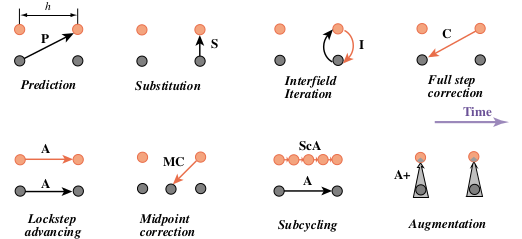
\includegraphics[width=\textwidth]{devices_of_partitioned_analysis_time_stepping.png}
  \caption{Devices of partitioned analysis time-stepping \citep{felippa_partitioned_2001}.}
\label{fig:devices_of_partitioned_analysis_time_stepping}
\end{figure}

Inter-field iterations are the primary criterion distinguishing loosely or one-way staggered coupled schemes and strongly or iterative staggered coupled schemes.
In the loosely coupled schemes, the integration algorithm proceeds sequentially, solving the problem in each field only once per time step.
On the other hand, for strongly coupled schemes, inter-field iterations are present, such that the problems are solved multiple times at the same time instant.
This inner loop is repeated until a given tolerance is reached for the unknowns in each field.

The remainder of the techniques listed will be mentioned and explained in the discussion below.

\subsection{Loosely coupled}



The solution for the fully coupled problem is found in loosely coupled schemes by solving each field sequentially.
For the thermomechanical problem, the two available schemes are the isothermal split (see e.g. \cite{simo_recent_1992}, \cite{agelet_de_saracibar_numerical_1998}) and the adiabatic split (see e.g. \cite{armero_new_1992} and \cite{armero_priori_1993}), as mentioned above.

According to \cite{felippa_partitioned_2001}, in linear problems, the first concern with partitioning is the degradation of time-stepping stability.
After the analyst has ensured stability, an accuracy analysis of the method should be performed.
In strongly nonlinear problems, such as fluid flow, stability and accuracy tend to be intertwined since numerical stability is harder to define.
As such, they are usually considered together in method design.
The expectation is for a method that operates well at a reasonable timestep.

\cite{felippa_partitioned_1988} present a detailed explanation about how to design from scratch a loosely coupled time-stepping algorithm applicable to linear systems of equations.
It includes implementation details, such as the choice of the predictor formula, and the design steps, from the formulation of the original field equations and temporal discretization to the stability and accuracy analysis.
Other contributions focused mainly on linear systems are \cite{neishlos_finite-element_1983}, \cite{zienkiewicz_unconditionally_1988} and \cite{combescure_numerical_2002},

Because the loosely coupled schemes are explicit, they are also often only conditionally stable.
The isothermic split is such an example \citep{armero_new_1992}.
On the other hand, the adiabatic split proposed in \cite{armero_new_1992} is unconditionally stable, despite being explicit.
\cite{farhat_unconditionally_1991} also propose a stable staggered scheme, achieved through semi-algebraic augmentation, which, however, is limited to linearized thermoelasticity.
In the context of coupled flow and geomechanics, \cite{kim_stability_2011-2} show that when the mechanical problem is solved first, the drained split combined with a backward Euler discretization is conditionally stable, and the undrained split is unconditionally stable when combined with midpoint rule.
When instead the flow problem is solved first, \cite{kim_stability_2011-1} show that the fixed-stress split is conditionally and the fixed-strain split is unconditionally stable for appropriate choices of the generalized midpoint rule.

Moreover, in the domain of fluid-structure interactions, it can be shown that staggered methods are inherently non-conservative.
As time progresses in the simulation, these schemes introduce parasitic energy at the boundary, which contributes to their poor numerical stability \citep{michler_relevance_2003}.
A further problem appears when solving these coupled physical problems, the so-called artificial added-mass effect, which leads to instability.
It manifests itself when a slender structure and fluid have similar densities, and the latter is modeled as an incompressible fluid \citep{causin_added-mass_2005, forster_robust_2007}.
It can even be shown that for every sequentially staggered scheme and spatial discretization of a problem, a mass ratio between the fluid and structural mass density can be found at which the coupled system becomes unstable \citep{forster_artificial_2007}.

Despite this, some contributions detail strategies allowing for the unconditional stability of these schemes.
As part of the development loop of commercial tire designs, \cite{gillard_efficient_2019} tackles the problem of tire hydroplaning.
The author presents a robust explicit coupling scheme that relies on rigorous control of the energy artificially introduced at the interface by the staggering process through a dynamic adaptation of the coupling time step size.
Regarding the artificial added-mass effect, \cite{farhat_robust_2010} demonstrates that even for fluid-structure applications with strong added mass effects, a carefully designed staggered and sub-iteration-free time-integrator can achieve numerical stability and robustness concerning the slenderness of the structure, as long as the fluid is justifiably modeled as a compressible medium.

Another technique available to improve the stability of loosely coupled schemes is (algebraic) augmentation.
It rests on the injection of one of the coupled equations into the other, after discretization in space, to 'soften' the system, either by reducing the large eigenvalues of the uncoupled stiff equation or by introducing some damping into it.
Some examples of this approach include \cite{park_stabilization_1977} and \cite{park_stabilization_1983}.

Yet another technique to ensure stability in the context of fluid-structure interactions is presented in \cite{fernandez_projection_2006}.
Stability is achieved employing a semi-implicit coupling scheme, splitting the added-mass, viscous effects, and geometrical/convective nonlinearities, through a Chorin-Temam projection scheme within the fluid.

Regarding accuracy, the loosely coupled schemes do not necessarily inherit the accuracy order of the schemes used in the integration of the separate fields, often being just of the first order in time \citep{farhat_provably_2006}.
However, some contributions detail approaches that are second-order time-accurate.
In the context of thermo-elasticity, \cite{armero_new_1992} show that a double-pass approach using the adiabatic split yields such a second-order accurate time-stepping algorithm.
A few approaches yield similar results in the domain of fluid-structure interaction (see \cite{piperno_explicitimplicit_1997}, \cite{farhat_provably_2006} and \cite{farhat_robust_2010}).
In any case, whatever the theoretical convergence order of the loosely coupled method, at a given time instant, the fully coupled discretized equations of the problem will never be exactly satisfied by the solutions found.
There is a lag between the fields considered, e.g., the mechanical and thermal fields in a thermomechanical problem.
In the context of strong coupling, this lag can be conceived as a numerical evaluation error.
Solving approximately the exact (i.e., aggregated) equations can be reinterpreted as exactly solving a set of approximate (i.e., segregated) equations.
Thus, one can construe loosely-coupled methods as solving a set of segregated equations instead of aggregated equations.
Accordingly, the incurred numerical evaluation error can be reinterpreted as a discretization error.
Loosely-coupled methods, therefore, satisfy conservation only in an asymptotic sense, i.e., for vanishing mesh width; this is a basic consistency requirement \citep{michler_efficient_2005}.

Prediction techniques can improve the order of the numerical evaluation error incurred by loosely-coupled partitioned methods.
For the sake of explanation, consider the thermo-mechanical problem being solved using the isothermic split.
When using predictors, instead of integrating the mechanical equations based on the structure's temperature in the previous time instant, a prediction can be used for the temperature of the structure boundary in the current time instant.
Such predictions are generally based on an extrapolation of the solution from the previous time step.
Prediction techniques improve the solution accuracy and stability of loosely-coupled methods \citep{piperno_explicitimplicit_1997, piperno_partitioned_2001, michler_efficient_2005, farhat_provably_2006}.

Another technique available to improve the accuracy of the loosely coupled methods is subcycling.
It involves solving each field's problems using different time steps since the fields present in a multi-physics problem often have different time scales.
In the context of aeroelasticity, \cite{piperno_partitioned_1995} claims that it can offer substantial computational advantages, including savings in the simulation CPU time because the structural field will be advanced fewer times.
\cite{farhat_high_1997} and \cite{piperno_explicitimplicit_1997} also argue for this technique along the same lines.

\paragraph{Usage examples}

The loosely coupled scheme has been used in the context of thermoelasticity \citep{argyris_natural_1981, armero_new_1992, johansson_thermoelastic_1993, miehe_entropic_1995, miehe_theory_1995, holzapfel_entropy_1996}, thermo-plasticity \citep{armero_new_1992, armero_priori_1993, simo_associative_1992, wriggers_coupled_1992, agelet_de_saracibar_numerical_1998, agelet_de_saracibar_formulation_1999} and thermo-viscoplasticity \citep{adam_numerical_2002, adam_numerical_2002-1}.

For examples in aeroelasticity see e.g., \cite{piperno_partitioned_1995, farhat_two_2000} and \cite{farhat_application_2003}, and in fluid-structure interaction more broadly see e.g. \cite{tezduyar2006space} and \cite{miller_loosely_2015}
Other applications include fluid-soil interaction analysis \citep{saetta_unconditionally_1992, armero_formulation_1999, mikelic_convergence_2013}.


\subsection{Strongly coupled}

In the strongly coupled scheme, inter-field iterations are performed until a given tolerance for the unknowns of each field is reached.
They converge to the solution of the monolithic scheme and are thus able to satisfy discrete versions of the coupled problem exactly \citep{forster_robust_2007, danowski_computational_2014}.
In principle, regarding thermomechanics, either the isothermal or the adiabatic slit can be used, but there seems to be no example of the latter.
In contrast to the staggered schemes, there is no problem of conditional stability, but the scheme may converge very slowly or not at all.
As an example coming from fluid-structure interactions, it has been shown that the number of coupling iterations increases when the time step decreases or when the structure becomes more flexible \citep{degroote_stability_2008}.
This can place a severe restriction on the use of these schemes.
Several acceleration techniques are available in the literature to speed up convergence.

A straightforward way to improve the convergence behavior of the strongly coupled schemes is using predictors, in contrast to the values found in the last step.
Thus, the initial guesses can be improved using well-chosen predictors \cite{michler_efficient_2005}.
Along these lines, \cite{erbts_accelerated_2012} employ polynomial prediction methods, and \cite{wendt_partitioned_2015} use a line extrapolation method to improve the first guess of the unknown and thus decrease the number of iterations needed to achieve convergence.

Another approach that is well established for series acceleration is the Aitken delta-squared process.
It uses previously computed values to obtain more accurate estimates for the unknown.
\cite{irons_version_1969} is an early contribution detailing this low-memory convergence acceleration scheme.
In the context of thermomechanics, \cite{danowski_computational_2014}, \cite{erbts_partitioned_2015} and \cite{wendt_partitioned_2015} use this technique, with the last authors also employing a quasi-Newton least squares method.
Some examples of contributions in the domain of fluid-structure interactions taking advantage of this approach are \cite{degroote_stability_2008}, \cite{kuttler_fixed-point_2008} and \cite{kuttler_vector_2009}.
The last authors also introduce a vector extrapolation approach that includes more than three previous values of the iteration scheme in the improved estimate.

The strongly coupled approach lends itself to an interpretation as a nonlinear block Jacobi or Gauss-Seidel scheme, whose convergence is conditional and at most linear \citep{matthies_strong_2003, joosten_analysis_2009}.
\cite{cervera_computational_1996} provides an in-depth analysis of block Jacobi and Gauss-Seidel schemes applied to coupled problems, including considerations regarding efficiency, complexity, and parallelization.
\cite{matthies_partitioned_2003, matthies_strong_2003} suggests a block-Newton method instead, with the Jacobian of the system being approximate by a finite difference method.
Under some assumptions on the subsystem solvers, this approach converges quadratically.
\cite{michler_interface_2005} propose a solution method based on the conjugation of sub-iterations via a Newton-Krylov method, which confines the GMRES acceleration to the interface degrees-of-freedom.
The latter renders storage requirements for the Krylov space and computational cost of the least-squares
problem low.
The nesting of Newton and GMRES iterations lends itself to the reuse of Krylov vectors in subsequent linear system solutions.
\cite{kuttler_vector_2009} claims that the approach proposed by the last authors should not be regarded as a Newton-based solver but as a Krylov-based vector extrapolation scheme

One can also improve the convergence speed of the strongly coupled scheme using reduced-order models to produce a more accurate first guess and thus decrease the number of iterations needed for the method to converge.
\cite{vierendeels_implicit_2007} presents a technique that uses the Jacobian from reduced-order models that are built up during the coupling iterations.
The reduced-order model is built for each step and approximates an arbitrary interface displacement fitting a linear regression to the previous displacement-stress points.
\cite{degroote_stability_2008} follows the same technique, coupling it with an Aitken delta-squared process.

\cite{blom_efficient_2017} proposes a manifold mapping technique to decrease the number of sub-iterations of a high-fidelity fluid-structure interaction model.
The idea is to perform many sub-iterations with a low-fidelity model instead of the high-fidelity flow and structure models.


\paragraph{Usage examples}

Regarding the use of strongly coupled schemes in the context of thermo-mechanics, there are a few contributions.
\cite{erbts_accelerated_2012} present results concerning thermo-elasticity at finite strains, \cite{netz_high-order_2013} concerning thermo-viscoelasticity, \cite{danowski_computational_2014} includes results on thermo-elasticity and thermo-elasto-plasticity.
In field of fluid-structure interaction, a few examples of the use of strongly coupled schemes are \cite{torii2006computer}, \cite{wall_strong_2007} and \cite{blom_efficient_2017}.
Including more than two fields, \cite{erbts_partitioned_2015} tackles electro-thermo-mechanical problems, as does \cite{wendt_partitioned_2015}, which also considers radiative heat transfer.
In \cite{lenarda_geometrical_2016}, the strongly coupled scheme is used to solve coupled hygro-thermo-mechanical problems in photovoltaic laminates.

\section{Comparison of solution techniques} \label{sec:comparison_sol_methods}

According to \cite{felippa_partitioned_1988}, the desirable properties of a time-stepping algorithm for solving coupled problems are:
\begin{itemize}
  \item enjoys unconditional stability;
  \item is highly accurate;
  \item is easy to implement;
  \item is not memory intensive;
  \item requires low CPU time;
  \item satisfies software modularity constraints.
  \end{itemize}
In the following, the time-stepping schemes presented above are compared with these criteria in mind.
The application in view is thermomechanics.

\paragraph{Stability}

Regarding stability, the loosely coupled using an isothermal split is conditionally stable \citep{armero_new_1992}.
Despite this, the limitation is not significant for metal plasticity, according to \cite{simo_associative_1992}.
However, examples where the scheme diverges, can be found in \cite{armero_new_1992}.
In this last contribution, the adiabatic split is introduced and shown to be unconditionally stable in the context of thermo-elasticity.
\cite{armero_priori_1993} show that these properties extend to thermo-plasticity.
The strongly coupled schemes are unconditionally stable because no critical time step leads to numerical instabilities in the results.
Despite this, the inner loop of the scheme may converge slowly or not at all \citep{matthies_strong_2003}.
It depends on the spectral radius of the matrices involved \citep{cervera_computational_1996}.
There are, however, acceleration techniques that can mitigate this problem, including predictors and Aitken \(\Delta^2\) methods (see Section~\ref{}).
\cite{danowski_computational_2014} presents a numerical example concerning an internal pressurized thick-walled cylinder, whose material is viscoplastic, for which the strongly coupled scheme employed diverged, despite the use of an Aitken method.
On the other hand, the monolithic scheme, as long as appropriately preconditioned, is unconditionally stable \citep{danowski_computational_2014}.

\paragraph{Accuracy}

Regarding accuracy, the solution found from the loosely coupled method will never exactly satisfy the fully coupled discretized equations of the problem.
There will be a time lag between the thermal and the mechanical field.
Loosely-coupled methods, therefore, satisfy conservation only in an asymptotic sense, i.e., for vanishing mesh width \citep{michler_efficient_2005}.
As long as it does not diverge, the monolithic and strongly coupled satisfy the coupled discretized equations exactly.

\paragraph{Ease of implementation}

The partitioned schemes are much easier to implement as most of them can work with the field analyzers as black boxes, concerning themselves only with communication between the solvers, initial guesses, and acceleration schemes using previously computed values.
The monolithic scheme requires the computation of the full stiffness matrix, including the mixed terms and appropriate preconditioning that varies widely with the specific multi-physics problem to be solved.

\paragraph{Memory requirements}

When it comes to memory requirements, the partitioned schemes often require only the diagonal blocks of the stiffness matrix found in the linearization process.
Previous values also need to be saved from one iteration to the next, increasing the memory cost for some acceleration techniques.
In contrast, the fully coupled monolithic scheme requires the full stiffness matrix of the coupled problem.

\paragraph{CPU time}

According to \cite{michler_efficient_2005}, solving a fluid-structure interaction problem with the same accuracy using a loosely and strongly coupled scheme, the latter is more efficient than the former.
For the same total number of iterations, the difference in the accuracy reached ranges from one to three orders of magnitude.
These results run counter to a claim in \cite{felippa_partitioned_2001}. However, this is not supported by any numerical results from the last authors.
In the numerical examples presented in \cite{danowski_computational_2014}, the monolithic solver is in most cases faster than a strongly coupled scheme employing an Aitken method for problems in thermomechanics.
The differences range from 120\% to 140\% in favor of the monolithic scheme.
Supporting evidence for these conclusions can also be found in \cite{novascone_evaluation_2015}.
The authors report  CPU time ratios between the strongly coupled and monolithic approaches, ranging from 0.635 to 3.75 on the magnitude of the coupling.

\paragraph{Software modularity}

The partitioned approaches can take full advantage of software, including closed source commercial solvers.
There is little to no software reuse for the monolithic approach, save for routines that solve linear systems and the like.

\paragraph{Conclusions}

Lastly, it may be helpful to reproduce the recommendations given in \cite{felippa_partitioned_2001} regarding the choice between partitioned and monolithic approaches.
According to the authors, the circumstances that favor the partitioned approach for tackling a coupled problem are a research environment with few delivery constraints, access to existing software, localized interaction effects (e.g., surface versus volume), and widespread spatial/temporal component characteristics.
The opposite circumstances:        commercial environment,        rigid deliverable timetable,        massive software development resources,        global interaction effects, and comparable length/time scales favors a monolithic approach.

Putting it all together, the most appropriate choice for the present use case is the strongly coupled schemes with appropriate acceleration techniques.
They can take advantage of already existing software, provide accurate results that agree with a monolithic approach, are not memory intensive, are easy to implement, and with the use of convergence acceleration techniques, are competitive from the computational efficiency standpoint.
The only drawback seems to be the possibility of divergence in the inner loop, stalling the progress of the simulation.

\begin{table}[htbp]
  \caption{Summary of the comparison between the FFT-Galerkin method.}
\label{tab:comparison_fft_galerkin_fem}
\small
  \setlength{\tabcolsep}{1pt}
  \centering
    \begin{tabular}{l ccc}
    & \multicolumn{2}{c}{Partitioned schemes} & \multirow{2}{*}{Monolithic} \\ \cline{2-3}
    & \vphantom{\Big |}Loosely coupled & Strongly coupled & \\
    \hline  \hline
    \vphantom{\Big |}Stability & \makecell[l]{Isothermic split:\\\ \textcolor{red!70!black}{conditionally stable}\\Adiabatic split:\\\ \textcolor{green!50!black}{unconditionally stable}} & \textcolor{green!50!black}{\makecell[c]{unconditionally\\stable\textsuperscript{*}}} & \textcolor{green!50!black}{\makecell[c]{unconditionally\\stable}}\\ \hline
    Accuracy & \textcolor{red!70!black}{\makecell[c]{Coupled discretized\\ equations not\\ satisfied exactly}} & \textcolor{green!50!black}{\makecell[c]{Coupled discretized\\ equations satisfied}} & \textcolor{green!50!black}{\makecell[c]{Coupled discretized\\ equations satisfied}} \\ \hline
    \makecell[l]{Ease of\\ implementation} & \multicolumn{2}{c}{\textcolor{green!50!black}{\makecell[c]{Only communication between field\\ analyzers stricly needed}}} & \makecell[l]{\textcolor{red!70!black}{Full coupling needed:}\\\ \textcolor{red!70!black}{\textbullet\ Computation of mixed}\\\ \textcolor{red!70!black}{terms of the Jacobian}\\\ \textcolor{red!70!black}{\textbullet\ Preconditioning needed}} \\ \hline
    \makecell[l]{Memory\\ requirements} & \multicolumn{2}{c}{\textcolor{green!50!black}{\makecell[c]{Only diagonal blocks of\\ the full stiffness matrix needed}}} & \textcolor{red!70!black}{Full stiffness matrix needed}\\ \hline
    \makecell[l]{Software modularity\\ constraints} & \multicolumn{2}{c}{\textcolor{green!50!black}{Full software modularity}} & \textcolor{red!70!black}{\makecell[c]{Poor or no\\ software modularity}}\\
  \hline\hline
  \multicolumn{4}{l}{\vphantom{\Huge |}\parbox{\textwidth}{\footnotesize{${}^*$ The inner loop of the strongly coupled scheme may converge very slowly or even diverge.}}}
  \end{tabular}
\end{table}

\newpage\null\thispagestyle{blank}\newpage

% \include{conclusions}
\appendix
% \include{annex}

\bibliography{Thermomechanics.bib}

\end{document}
